In this section, we demonstrate the performance of pyMIC2 by comparing functions implemented in pyMIC2 to those of NumPy. We then evaluate MNIST handwritten digit recognition application by using a deep learning framework called Chainer. This application is a classical one in machine learning. The core computing library of Chainer is NumPy, and we want to replace it with pyMIC2 to see how well pyMIC2 works in comparison to NumPy so that we can prove that our approach is practical and efficient enough. Before discussing all of that, we first consider the environment and system on which our experiments are conducted.

\subsection{System Setup}
In this paper, all of the experiments are conducted on a compute node that has 128 GB RAM, two-way processor Intel Xeon CPU E5-2680 v3 @ 2.50GHz about 1 TFLOPS and 2 first generation Intel Xeon Phi coprocessors 7120 series connected through PCIe with 1.2 TFLOPS each card.

Furthermore, in order to utilize all computing power of Intel Xeon Phi coprocessor, all threads must be used. However, threads can migrate from one core to another, which is depending on OS scheduling decisions. This leads to performance depletion because migrated threads must fetch data into cache of a new core \cite{colfaxbook}. Among all of the optimization techniques on Intel Xeon Phi, there is one called thread affinity. We can inhibit thread migration by setting environment variable KMP\_AFFINITY to scatter, compact, or several other modes \cite{threadaffinity}, and two of the most popular are scatter and compact. The former is especially good for memory and the latter is for computing.

Moreover, we can improve data transfer performance by using huge memory pages. When data offloaded to coprocessor exceed a threshold value set to MIC\_USE\_2MB\_BUFFERS, memory will be allocated on big 2MB pages, by default the size of pages on Intel Xeon Phi is 4KB. Therefore, we can access more data with less pages, which will decrease page fault rate \cite{bigmempage}. There is also a lower allocation cost.

%[https://software.intel.com/en-us/mkl-linux-developer-guide-improving-performance-on-intel-xeon-phi-coprocessors].

In summary, to achieve the best performance, our system is configured to KMP\_AFFINITY=compact, MIC\_USE\_2MB\_BUFFERS=16K. Additionally,  all of our benchmarks are run 100 times.

%, and any jitter will be removed to guarantee the accuracy of all benchmarks.

\subsection{Evaluation of computing functions in pyMIC2}
NumPy with easy-to-use Python API is a big, high performance computing library and has been developed and updated for a decade. In pyMIC2, we only implement several unit functions that mainly support deep learning. We divide these into three group (Table \ref{list-func}):
\begin{itemize}
	\item The first group is related to logical operations.
	\item The second group is about arithmetic, exponential and logarithmic functions. 
	\item The final group only consists of 1 function which is matrix multiplication function. This is a one of the important benchmarks in LINPACK used to measure the performance for a given machine.
\end{itemize}

%\begin{table}[]
%\centering
%\caption{My caption}
%\label{my-label}
%\begin{tabular}{|c|c|c|}
%\hline
%\multicolumn{2}{|c|}			{\multirow{4}{*}{Group 1}} 		& EQ \\ \cline{3-3} 
%\multicolumn{2}{|c|}{}                         				& GT \\ \cline{3-3} 
%\multicolumn{2}{|c|}{}                         				& NE \\ \cline{3-3} 
%\multicolumn{2}{|c|}{}                         				& OR \\ \hline
%\multirow{17}{*}{Group 2} 	& \multirow{9}{*}{Subgroup 1} 	& ABS \\ \cline{3-3}
%\multirow{17}{*}{} 			& \multirow{9}{*}{} 				& MEAN \\ \cline{3-3}
%\multirow{17}{*}{} 			& \multirow{9}{*}{} 				& SUM axis=0 \\ \cline{3-3}
%\multirow{17}{*}{} 			& \multirow{9}{*}{} 				& SUM axis=1 \\ \cline{3-3}
%\multirow{17}{*}{} 			& \multirow{9}{*}{} 				& SUM axis=None \\ \cline{3-3}
%\multirow{17}{*}{} 			& \multirow{9}{*}{} 				& ARGMAX axis=1 \\ \cline{3-3}
%\multirow{17}{*}{} 			& \multirow{9}{*}{} 				& ADD 2 shape-equal arrays  \\ \cline{3-3}
%\multirow{17}{*}{} 			& \multirow{9}{*}{} 				& SUB 2 shape-equal arrays\\ \cline{3-3}
%\multirow{17}{*}{} 			& \multirow{9}{*}{} 				& MUL 2 shape-equal arrays \\ \cline{2-3}
%\multirow{17}{*}{} 			& \multirow{5}{*}{Subgroup 2} 	& ARANGE \\ \cline{3-3}
%\multirow{17}{*}{} 			& \multirow{5}{*}{} 				& MAXIMUM \\ \cline{3-3}
%\multirow{17}{*}{} 			& \multirow{5}{*}{} 				& LOG \\ \cline{3-3}
%\multirow{17}{*}{} 			& \multirow{5}{*}{} 				& EXP \\ \cline{3-3}
%\multirow{17}{*}{} 			& \multirow{5}{*}{} 				& ARGMAX axis=0 \\ \cline{2-3}
%\multirow{17}{*}{} 			& \multirow{3}{*}{Subgroup 3} 	& ADD 2 shape-different arrays \\ \cline{3-3}
%\multirow{17}{*}{} 			& \multirow{3}{*}{} 				& SUB 2 shape-different arrays\\ \cline{3-3}
%\multirow{17}{*}{} 			& \multirow{3}{*}{} 				& MUL 2 shape-different arrays\\ \hline
%\multicolumn{2}{|c|}			{Group 3} 						& MATRIX MULTIPLICATION \\ \hline
%\end{tabular}
%\end{table}

\begin{table}[]
\centering
\caption{List of computing functions}
\label{list-func}
\begin{tabular}{|c|c|}
\hline
\multirow{4}{*}{Group 1} 					& EQ \\ \cline{2-2} 
\multirow{4}{*}{}                         	& GT \\ \cline{2-2} 
\multirow{4}{*}{}                         	& NE \\ \cline{2-2} 
\multirow{4}{*}{}                         	& OR \\ \hline

\multirow{17}{*}{Group 2} 	 				& ABS \\ \cline{2-2}
\multirow{17}{*}{} 							& MEAN \\ \cline{2-2}
\multirow{17}{*}{} 							& SUM axis=0 \\ \cline{2-2}
\multirow{17}{*}{} 							& SUM axis=1 \\ \cline{2-2}
\multirow{17}{*}{} 			 				& SUM axis=None \\ \cline{2-2}
\multirow{17}{*}{} 			 				& ARGMAX axis=1 \\ \cline{2-2}
\multirow{17}{*}{} 							& ADD 2 shape-equal arrays  \\ \cline{2-2}
\multirow{17}{*}{} 							& SUB 2 shape-equal arrays\\ \cline{2-2}
\multirow{17}{*}{} 							& MUL 2 shape-equal arrays \\ \cline{2-2}
\multirow{17}{*}{} 				 			& ARANGE \\ \cline{2-2}
\multirow{17}{*}{} 							& MAXIMUM \\ \cline{2-2}
\multirow{17}{*}{} 							& LOG \\ \cline{2-2}
\multirow{17}{*}{}		 					& EXP \\ \cline{2-2}
\multirow{17}{*}{} 							& ARGMAX axis=0 \\ \cline{2-2}
\multirow{17}{*}{}  							& ADD 2 shape-different arrays \\ \cline{2-2}
\multirow{17}{*}{} 		 					& SUB 2 shape-different arrays\\ \cline{2-2}
\multirow{17}{*}{} 		 					& MUL 2 shape-different arrays\\ \hline

Group 3 										& MATRIX MULTIPLICATION \\ \hline
\end{tabular}
\end{table}

%In each group, there will be a few graphs that represent for the whole group, and a table which contains execution time of all the functions in that group. The reason we do that because the appearance of graphs of all functions looks almost the same, and cannot be distinguished by naked eyes.Therefore, beside graphs, we have a table.

Input data to pyMIC2 functions can be an 1 or 2 two-dimension arrays or none, which is depending on operations. Size of all the dimensions is equal to N that increases from 128 to 16384. Furthermore, each element of an array is a 64-bit number which can be integer or float. In each benchmark, there are three lines:
\begin{itemize}
	\item The blue one represents for execution time of a NumPy function.
	\item The orange one is for pyMIC2 kernel, which is the time only for computing.
	\item The grey one is for computing time and transferring data.
\end{itemize}

\subsubsection{Group 1}

%In the first group, there are 4 functions of logical operations (table \ref{tab:group1}). When you look at graph of EQ function (figure \ref{fig:func-or}), the pymic line is time-comsuming because of data transfering through PCIe. The others two nearly take the same amount of time to finish the job, when N is approximately smaller than 9000. However, when N gets bigger, pymic kernel takes less time to finish in comparison to numpy. This happens the same for other functions, when we look at table \ref{tab:group1}.

In the first group, there are 4 functions of logical operations. The pymic line is time-consuming because of data transferring through PCIe. The other two nearly take the same amount of time to finish the job, when N is approximately smaller than 9000. However, when N gets bigger, pymic kernel takes less time to finish in comparison to numpy.
\begin{figure}[]
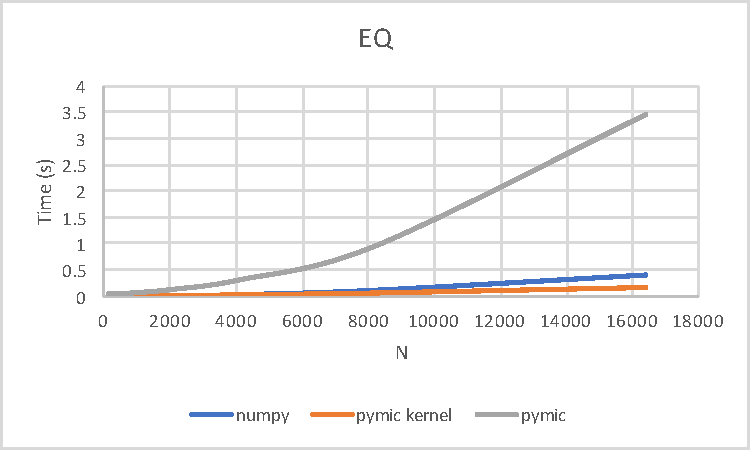
\includegraphics[scale=0.5]{img/group1/eq.pdf}
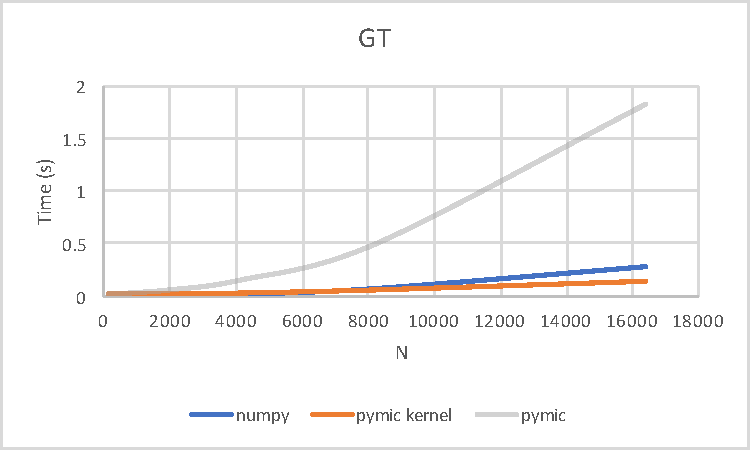
\includegraphics[scale=0.5]{img/group1/gt.pdf}
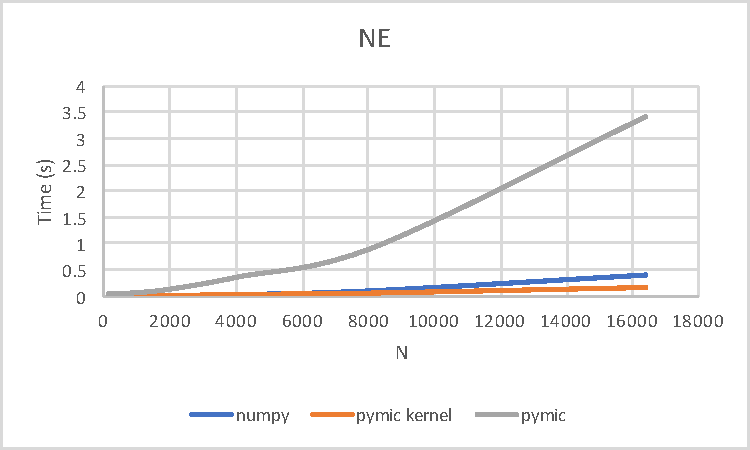
\includegraphics[scale=0.5]{img/group1/ne.pdf}
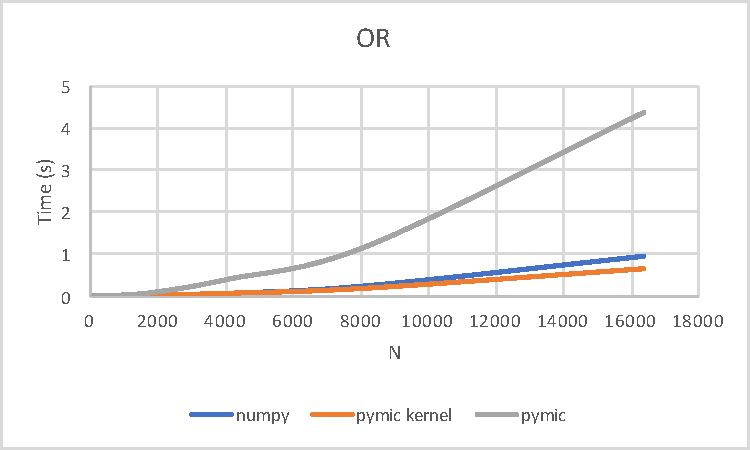
\includegraphics[scale=0.5]{img/group1/or.pdf}
\caption{Benchmark of group 1}
\label{fig:func-or}
\end{figure}

%\begin{table}[]
%\centering
%\caption{Time execution of Group 1}
%\label{tab:group1}
%\resizebox{\textwidth}{!}{\begin{tabular}{|c|c|c|c|c|c|c|c|c|c|c|c|}
%\hline
%
%\multirow{13}{*}{Group 2} 	& Function 	& Size & 128 & 256 & 512 & 1024 & 2048 & 4096 & 8192 & 16384 \\ \cline{2-11}
%
%\multirow{13}{*}{} 			& \multirow{3}{*}{EQ} 	& Numpy & 0.00004 & 0.00006 & 0.00019 & 0.00065 & 0.00532 & 0.02188 & 0.10596 & 0.39615\\
%\multirow{13}{*}{} 			& \multirow{3}{*}{} 		& PyMIC kernel & 0.02835 & 0.03057 & 0.02829 & 0.0284 & 0.03016 & 0.04298 & 0.07092 & 0.15468 \\
%\multirow{13}{*}{} 			& \multirow{3}{*}{} 		& PyMIC & 0.03565 & 0.03695 & 0.03747 & 0.05694 & 0.11581 & 0.29955 & 0.94572 & 3.46047 \\ \cline{2-11}
%
%\multirow{13}{*}{} 			& \multirow{3}{*}{GT} 	& Numpy & 0.00003 & 0.00007 & 0.00029 & 0.00111 & 0.00385 & 0.01717 & 0.07109 & 0.28695 \\
%\multirow{13}{*}{} 			& \multirow{3}{*}{}	 	& PyMIC kernel & 0.02772 & 0.02794 & 0.0277 & 0.02795 & 0.02828 & 0.03334 & 0.06056 & 0.13563\\
%\multirow{13}{*}{} 			& \multirow{3}{*}{} 		& PyMIC & 0.03008 & 0.03143 & 0.03248 & 0.04231 & 0.06886 & 0.15801 & 0.49964 & 1.82656\\ \cline{2-11}
%
%\multirow{13}{*}{} 			& \multirow{3}{*}{NE} 	& Numpy & 0.00003 & 0.00006 & 0.0003 & 0.00069 & 0.00592 & 0.02441 & 0.10494 & 0.42276\\
%\multirow{13}{*}{} 			& \multirow{3}{*}{}	 	& PyMIC kernel & 0.02768	& 0.02471 & 0.02796 & 0.02835 & 0.02826 & 0.04767 & 0.07064 & 0.16073 \\
%\multirow{13}{*}{} 			& \multirow{3}{*}{} 		& PyMIC & 0.03313 & 0.03069 & 0.0371 & 0.05222 & 0.12364 & 0.35599 & 0.92778 & 3.42537\\ \cline{2-11}
%
%\multirow{13}{*}{} 			& \multirow{3}{*}{OR} 	& Numpy & 0.00008 & 0.00032 & 0.00045 & 0.00254 & 0.01586 & 0.06144 & 0.24561 & 0.97365\\
%\multirow{13}{*}{} 			& \multirow{3}{*}{}	 	& PyMIC kernel & 0.02784 & 0.02825 & 0.03033 & 0.03554 & 0.04832 & 0.08806 & 0.20858 & 0.66821\\
%\multirow{13}{*}{} 			& \multirow{3}{*}{} 		& PyMIC & 0.03524 & 0.03544 & 0.03951 & 0.05648 & 0.1325 & 0.42557 & 1.20206 & 4.36309\\ \hline
%
%\end{tabular} }
%\end{table}

\subsubsection{Group 2}
%The second group consists of functions of arithmetic, exponent and logarithm. As usually, pymic line is the slowest. The two other lines can be almost equal, or one can run faster than another and vice versa. For better clarification. We will have three subgroup.
%
%\begin{itemize}
%\item In subgroup 1, the pymic kernel line is approximately equal to numpy. It consists of 9 functions
%
%\item The next subgroup consist 5 functions that runs faster than those of numpy. In arange graph, at first numpy achieves better result than pymic kernel, but when N is getting larger, pymic starts to catch up and runs faster than numpy. The benchmark results of function exp and log are quite interesting, pymic line in exp is almost equal when N is less than 6000, while pymic line in log graph is much faster than numpy. The reason is that for functions such as exponent and logarithm, Intel Compiler includes a mathematical software library containing highly optimized and very accurate mathematical functions, commonly used in scientific or graphic applications [https://software.intel.com/en-us/node/522653].
%
%
%\item Finally,we have three functions that do not run as good as numpy functions. Although, when N gets bigger than N 7500, they starts to works as efficiently as those of numpy.  
%\end{itemize}
%%%%%%%%%%
The second group consists of functions of arithmetic, exponent and logarithm. As usual, pymic line of most functions is the slowest, but when N is getting larger, pymic starts to work more efficient and runs faster than numpy. However, there are still some exceptional functions:

\begin{figure}
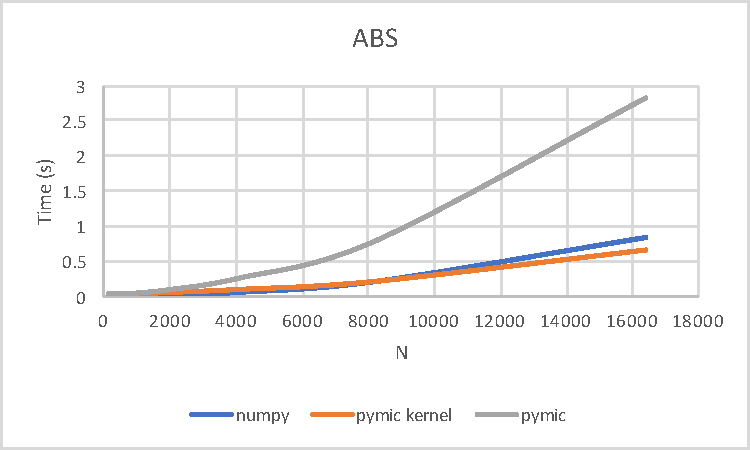
\includegraphics[scale=0.5]{img/group2/abs.pdf}
\includegraphics[scale=0.5]{{"img/group2/argmax axis1"}.pdf}
\end{figure}

\begin{figure}
\centering
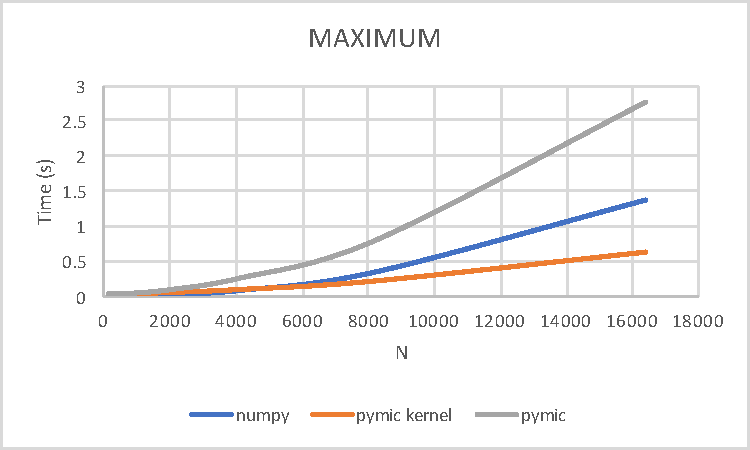
\includegraphics[scale=0.5]{img/group2/maximum.pdf}
\end{figure}

\begin{figure}[]
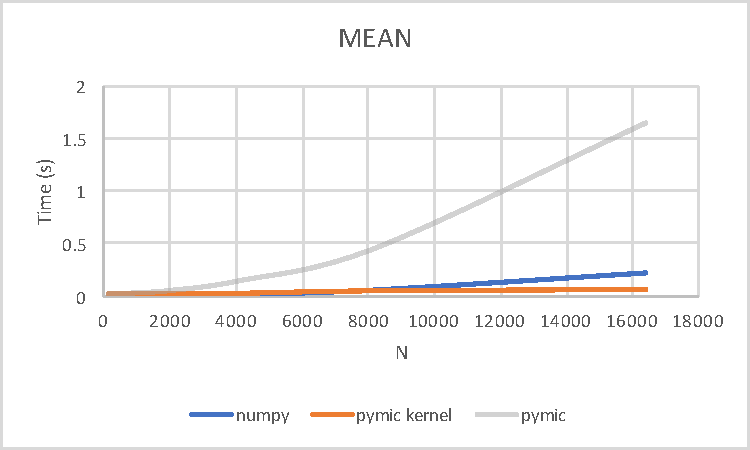
\includegraphics[scale=0.5]{img/group2/mean.pdf}
\includegraphics[scale=0.5]{{"img/group2/sum axis0"}.pdf}
\end{figure}

\begin{figure}[]
\includegraphics[scale=0.5]{{"img/group2/sum axis1"}.pdf}
\includegraphics[scale=0.5]{{"img/group2/sum axisNone"}.pdf}
\end{figure}

\begin{figure}[]
\includegraphics[scale=0.5]{{"img/group2/add same shape"}.pdf}
\includegraphics[scale=0.5]{{"img/group2/add diff shape"}.pdf}
\end{figure}

\begin{figure}[]
\includegraphics[scale=0.5]{{"img/group2/sub same shape"}.pdf}
\includegraphics[scale=0.5]{{"img/group2/sub diff shape"}.pdf}
\end{figure}

\begin{figure}[]
\includegraphics[scale=0.5]{{"img/group2/mul diff shape"}.pdf}
\includegraphics[scale=0.5]{{"img/group2/mul same shape"}.pdf}
\end{figure}

\begin{itemize}
	\item Function ARGMAX axis=0
	\item Fucntion ARANGE
	\item Function EXP and LOG
\end{itemize}

In function ARANGE, pymic line and numpy are approximately the same because it requires no data transferred to coprocessor. Beside function ARANGE, the numpy line of all functions mentioned above is slower than pymic line which includes transferring time. The results of function EXP and LOG can be explained that for exponential and logarithmic functions, Intel Compiler includes a mathematical software library containing highly optimized and very accurate mathematical functions, commonly used in scientific or graphic applications \cite{mathlib}.

\begin{figure}[]
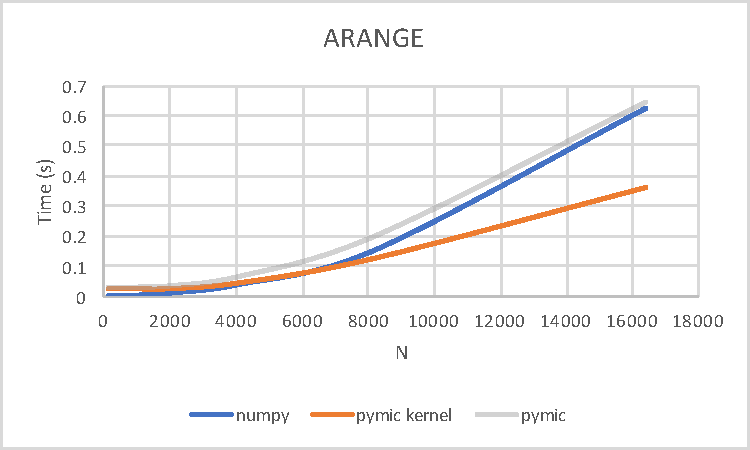
\includegraphics[scale=0.5]{img/group2/arange.pdf}
\includegraphics[scale=0.5]{{"img/group2/argmax axis0"}.pdf}
\end{figure}

\begin{figure}[]
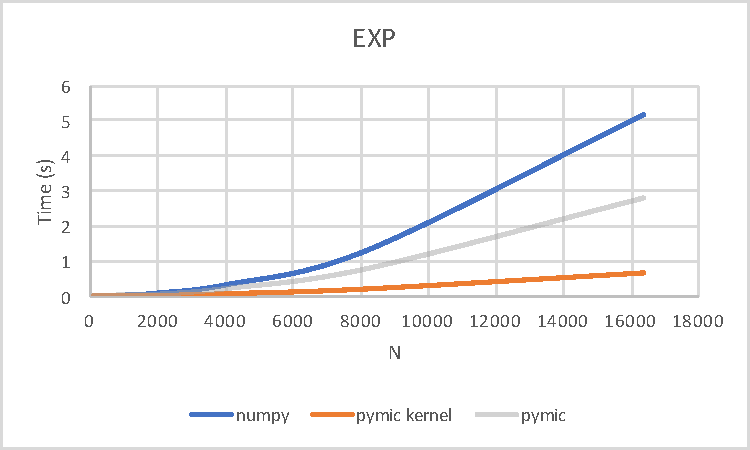
\includegraphics[scale=0.5]{img/group2/exp.pdf}
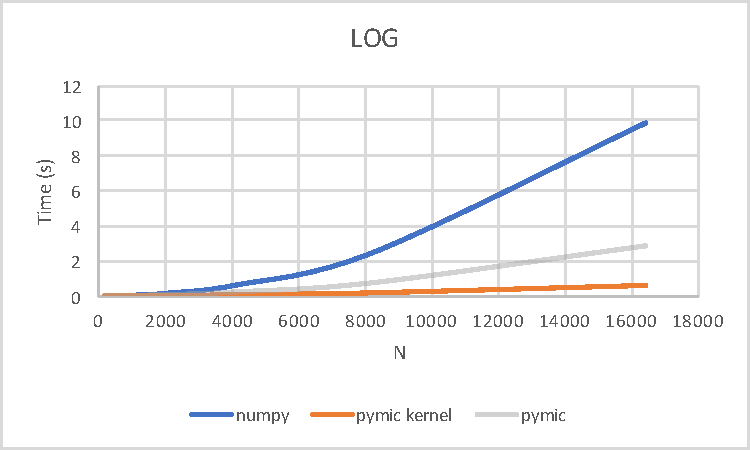
\includegraphics[scale=0.5]{img/group2/log.pdf}
\end{figure}

\subsubsection{Group 3}
In the final group, we use FLOPS (floating point operation per second) for matrix multiplication benchmark instead of time so that we can know how faster this function can achieve in comparison to theoretical performance. This function in pymic will call one of functions of Intel Math Kernel Library (MKL). General matrix multiplication of Intel MKL has been optimized for Intel architecture and proved the efficiency even for small size. 

In Fig. \ref{fig:func-dot}, we can see that peak performance of numpy, pymic kernel and pymic lines are 574, 849 and 596 GLOPS respectively. For small size matrix, numpy works more efficiently than pymic kernel, but pymic kernel starts to outperform numpy when N is greater than 2500. As pymic kernel, pymic also runs faster than numpy when N is greater than 13000. The computation time of pymic can compensate its transferring time, which leads to better performance than Numpy. Moreover, without including transferring overhead, pymic kernel runs 200 GFLOPS faster than pymic

\begin{figure}[]
\centering
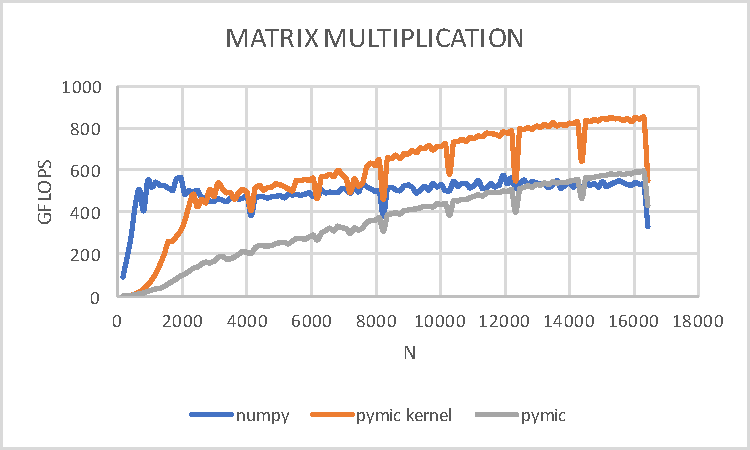
\includegraphics[scale=0.7]{img/dot128.pdf}
\caption{Matrix Multiplication}
\label{fig:func-dot}
\end{figure}